\documentclass{ximera}

%\addPrintStyle{..}

\begin{document}
	\author{Bart Lambregs}
	\xmtitle{Eenparige rechtlijnige beweging}{}
    \xmsource\xmuitleg




Een eenvoudige beweging om te bestuderen is de \emph{eenparig rechtlijnige beweging} (afgekort ERB). 
De snelheid van de beweging is eenparig\footnote{Van Dale: zonder onderling verschil; gelijk} of gelijkmatig verdeeld wat betekent dat de snelheid steeds gelijk blijft. 
De snelheid is m.a.w. constant en dus de versnelling gelijk aan nul. 
Aangezien de snelheid niet verandert is de ogenblikkelijke snelheid gelijk aan de gemiddelde snelheid. 
Met deze observatie kan je eenvoudig een functie opstellen voor de plaatsfunctie van deze beweging:

\[
\begin{array}{rcl}

v=\frac{\Delta x}{\Delta t} & \Leftrightarrow & \Delta x=v\Delta t \\
&\Leftrightarrow & x-x_0=v(t-t_0) \\
&\Leftrightarrow & x=x_0+v(t-t_0)

\end{array}
\]

\begin{theorem}
De plaatsfunctie $x(t)$ van een ERB met snelheid $v$ is gegeven door:

\[
x(t)=x_0+v(t-t_0)
\]
waarbij $x_0=x(t_0)$ de coördinaat op het tijdstip $t_0$ is. Als $t_0=0$ dan vereenvoudigt de plaatsfunctie tot
\begin{eqnarray}%
x(t)&=&x_0+vt
\end{eqnarray}

De snelheid $v$ is gelijk aan de beginsnelheid $v_0=v(t_0)$ omdat in een ERB de snelheid constant is. De snelheidsfunctie is $v(t)=v$ en de versnellingsfunctie is $a(t)=0$.

\begin{image}
	
    \begin{tikzpicture}
		\begin{scope}[shift={(0,4)}]
			\draw[->] (0,0) -- (4,0) node[right] {$t$};
			\draw[->] (0,-1.5) -- (0,2.5) node[above] {$x$};

			\draw[dashed] (0,1) -- (3.5,2.5);
			\draw[thick]  (0,0) -- (3.5,1.5);
			\draw[dashed] (0,-1) -- (3.5,0.5);

			\node[left] at (0,1) {$x_0>0$};
			\node[left] at (0,0) {$x_0=0$};
			\node[left] at (0,-1) {$x_0<0$};
		\end{scope}
			
		\begin{scope}[shift={(6,5)}]

			\draw[->] (0,0) -- (4,0) node[right] {$t$};
				\draw[->] (0,-2.5) -- (0,1.5) node[above] {$x$};

				\draw[dashed] (0,1) -- (3.5,-0.5);
				\draw[thick]  (0,0) -- (3.5,-1.5);
				\draw[dashed] (0,-1) -- (3.5,-2.5);

				\node[left] at (0,1) {$x_0>0$};
				\node[left] at (0,0) {$x_0=0$};
				\node[left] at (0,-1) {$x_0<0$};
		\end{scope}
	
		\begin{scope}[shift={(0,0)}]

			\draw[->] (0,0) -- (4,0) node[right] {$t$};
			\draw[->] (0,-1) -- (0,1.2) node[above] {$v$};

			\draw[thick] (0,0.6) -- (3.5,0.6);

			\node at (2,0.8) {$v>0$};
		\end{scope}
		
		\begin{scope}[shift={(6,0)}]

			\draw[->] (0,0) -- (4,0) node[right] {$t$};
			\draw[->] (0,-1.2) -- (0,1) node[above] {$v$};

			\draw[thick] (0,-0.6) -- (3.5,-0.6);

			\node at (2,-0.8) {$v<0$};
		\end{scope}
		
	\end{tikzpicture}

\end{image}
\captionof{figure}{Grafieken van de ERB}


\end{theorem}




% \begin{image}
% 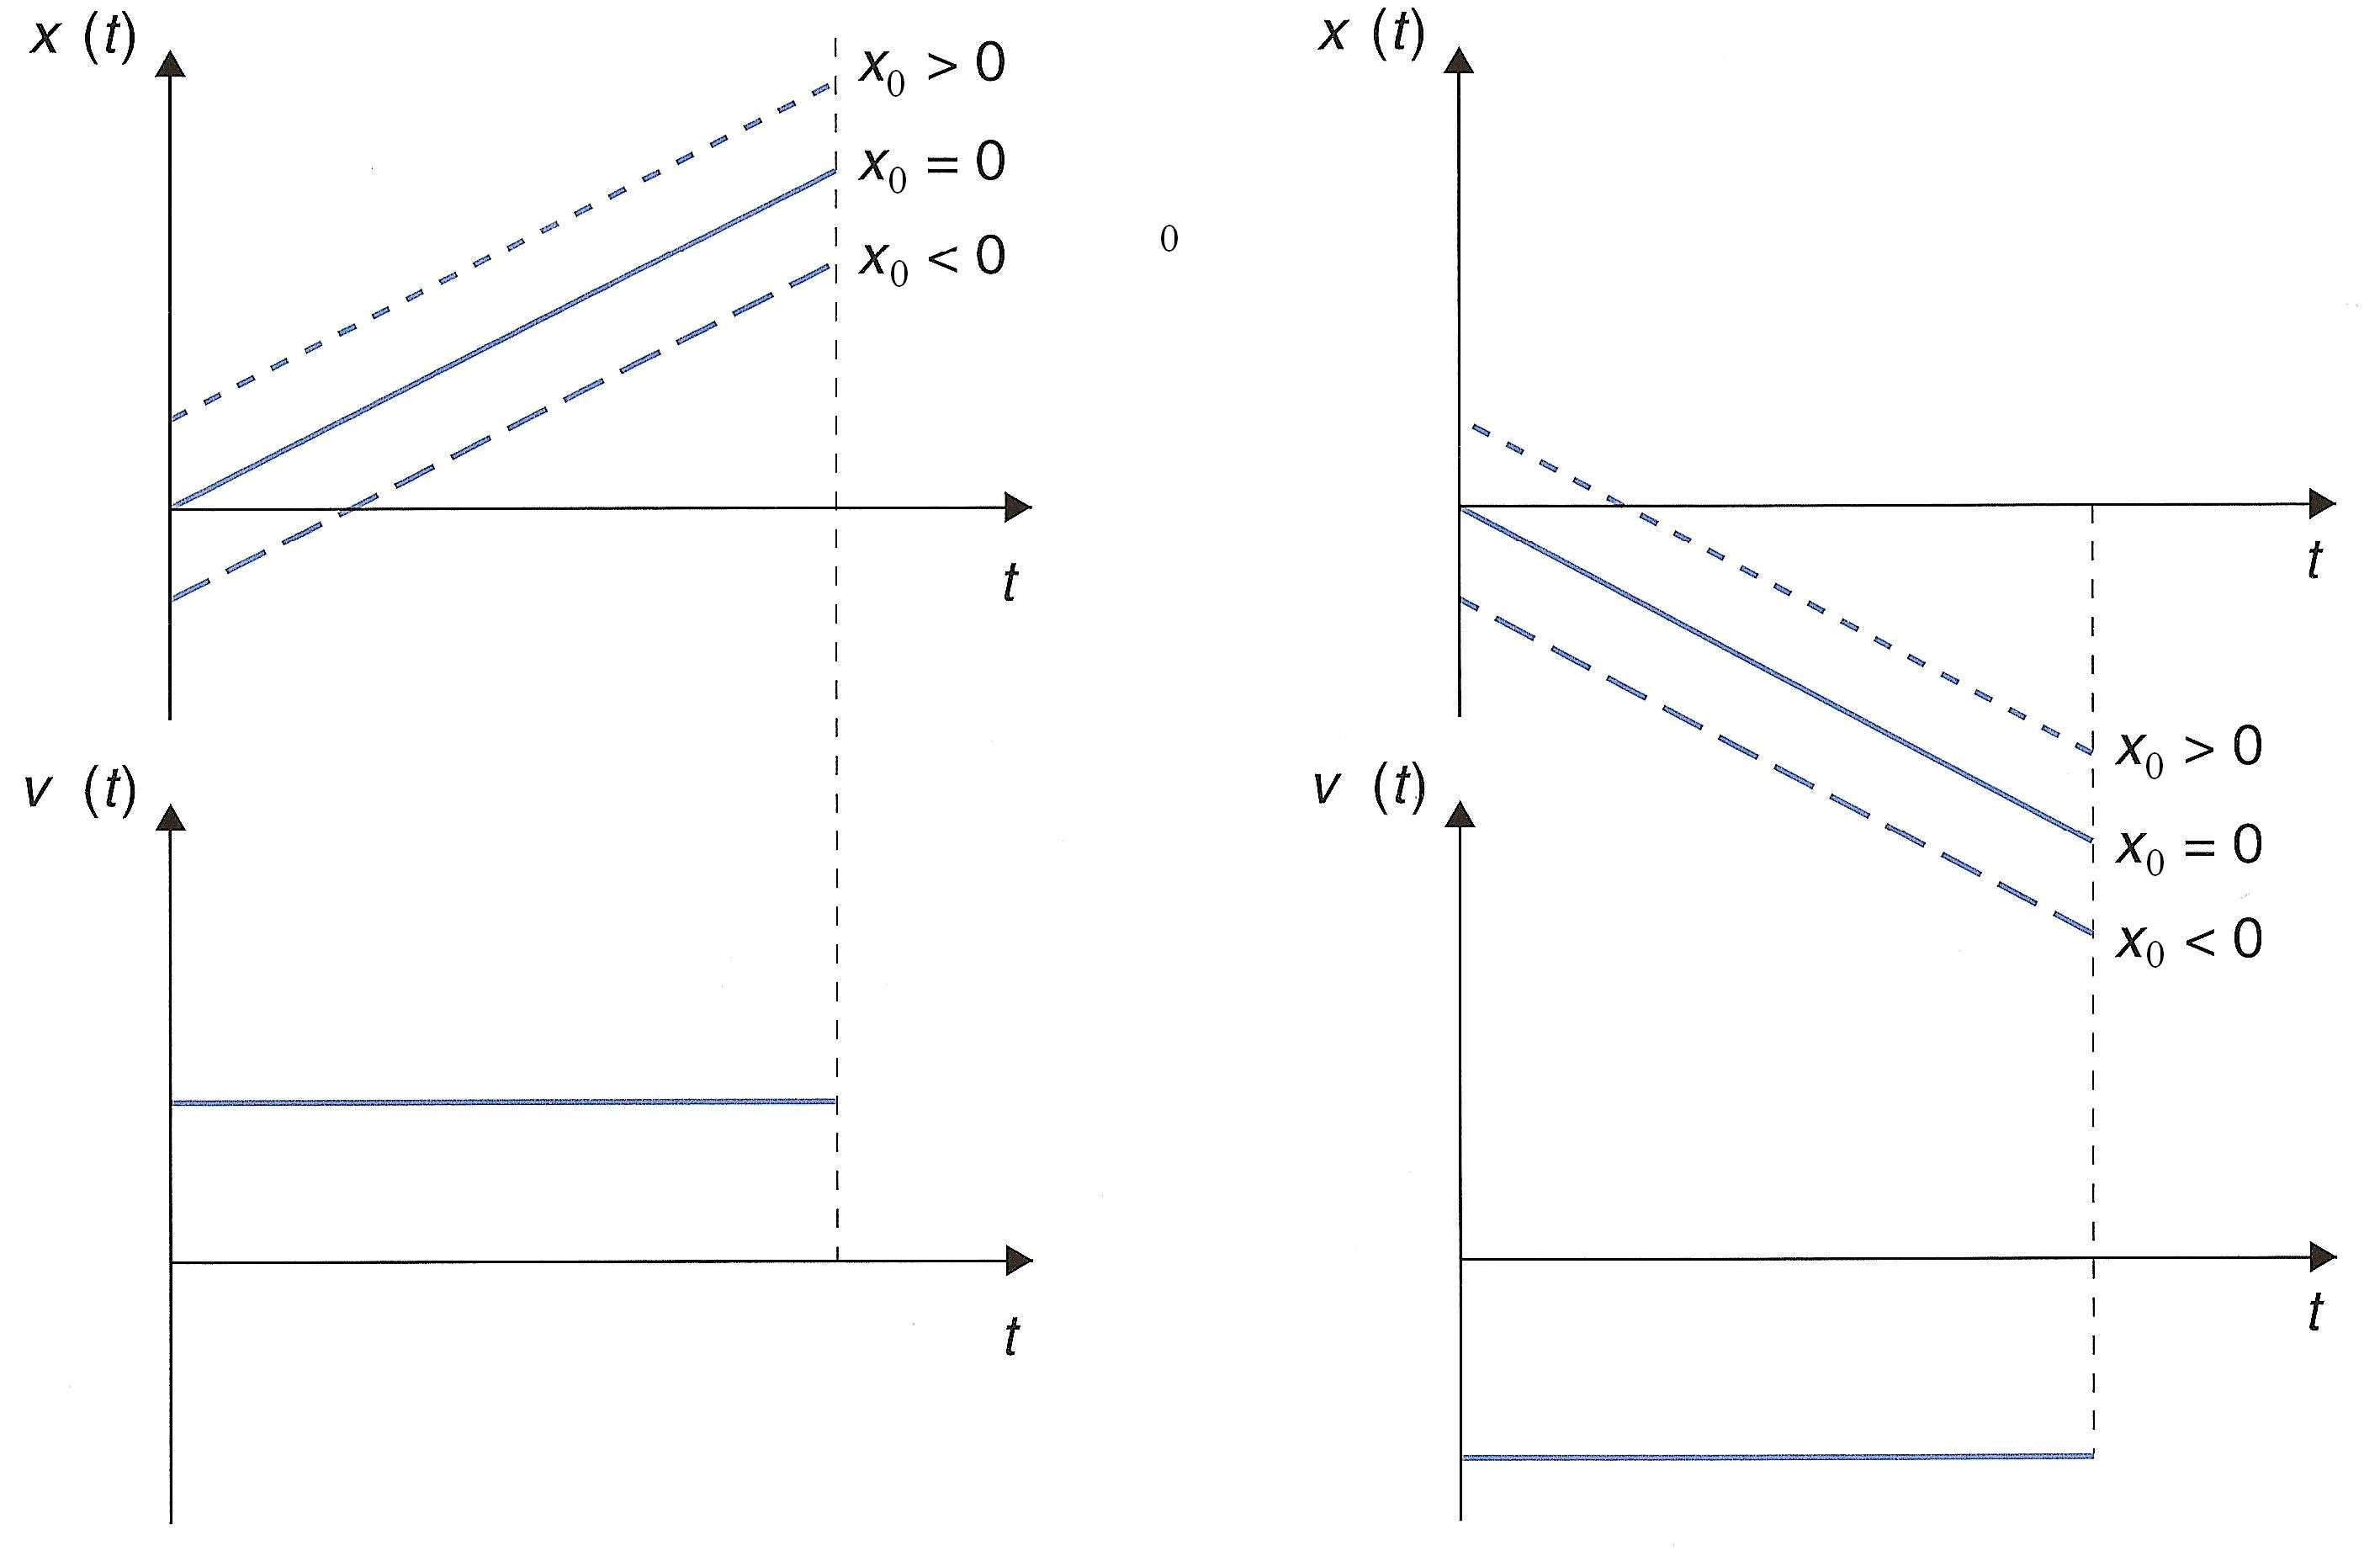
\includegraphics[width=.7\textwidth]{ERB_grafieken}
% \end{image}
% \captionof{figure}{Grafieken van een ERB}



\end{document}
